\documentclass{beamer}
\usepackage[utf8]{inputenc}
\usepackage{amsmath,amsfonts,amsthm,amstext,amssymb, xcolor, tikz, pgf}

% ----------------------------------------------------------
% Theme Setup

% Use Metropolis Theme
\usetheme[numbering=fraction]{metropolis}
\setbeamertemplate{blocks}[rounded][shadow=false]
\makeatletter
\setlength{\metropolis@titleseparator@linewidth}{1pt}
\makeatother

% Define Colors
\definecolor{chargerblue}{HTML}{002764}
\definecolor{chargerred}{HTML}{e02034}
\definecolor{bggray}{HTML}{d0d3d4}

% Set Colors
\setbeamercolor{title}{fg=chargerblue}
\setbeamercolor{background canvas}{bg=white}
\setbeamercolor{title separator}{fg=chargerred}
\setbeamercolor{structure}{fg=chargerblue}
\setbeamercolor{frametitle}{fg=white, bg=chargerblue}
\setbeamercolor*{normal text}{fg=chargerblue}
\setbeamercolor*{block body}{bg=bggray}
\setbeamercolor*{block title}{bg=chargerblue, fg=white}
% ----------------------------------------------------------

% ----------------------------------------------------------
% Custom Definitions, Commands, Environments, etc.

% Sets of numbers
\def\R{\mathbb{R}} % The reals
\def\N{\mathbb{N}} % The naturals
\def\Z{\mathbb{Z}} % The integers
\def\Q{\mathbb{Q}} % The rationals

% Blank space
\newcommand{\blank}[1]{\underline{\hspace{#1}}} % Blank space

% Fitted inclusion symbols
\newcommand{\fp}[1]{\left({#1}\right)} % Fitted parentheses around content
\newcommand{\fb}[1]{\left[{#1}\right]} % Fitted brackets
\newcommand{\set}[1]{\left\{{#1}\right\}} % Fitted braces (useful for sets)
\newcommand{\av}[1]{\left|{#1}\right|} % Fitted absolute value bars



% Coordinate Plane (Four-Quadrant)
\def\coordplane {
	\begin{tikzpicture}		\draw[step=0.25cm,black,very thin,opacity=0.25] (-2.5cm, -2.5cm) grid (2.5cm, 2.5cm);
		\draw[<->,thick,black] (-2.5cm, 0) -- (2.5cm, 0) node[anchor=north west,pos=0.94,font=\scriptsize]{$x$};
		\draw[<->,thick,black] (0,-2.5cm) -- (0, 2.5cm) node[anchor=south east,font=\scriptsize,pos=0.94]{$y$};
	\end{tikzpicture}
}

% Coordinate Plane (One-Quadrant)
\def\onequad {
	\begin{tikzpicture}
		\draw[step=0.25cm, black, very thin, opacity=0.25] (0,0) grid (7.5cm,5cm);
		\draw[->, thick, black] (0,0) -- (7.5cm, 0) node[anchor=north west,font=\scriptsize,pos=0.94]{$x$};
		\draw[->, black, thick] (0,0) -- (0,5cm) node[anchor=south east,font=\scriptsize,pos=0.94]{$y$};
	\end{tikzpicture}
}
% ----------------------------------------------------------

% ----------------------------------------------------------
% Presentation Information 
\title[P.3 and P.4]{Polynomials and Factoring}
\subtitle{Sections P.3 and P.4}
\author{Jacob Ayers}
\institute{Lesson \# 2}
\date{MAT 130}
% ----------------------------------------------------------

\begin{document}

% Slide 1 (Title Slide)
\begin{frame}
\titlepage
\end{frame}

% Slide 2 (Objectives)
\begin{frame}[t]{Objectives}
\begin{itemize}
	\item Find the degree and leading coefficient of a polynomial
	\item Add, subtract, and multiply polynomials
	\item Compute special products of polynomials
	\item Factor polynomials by factoring out common factors
	\item Factor special polynomial forms
	\item Factor by grouping
	\item Factor trinomials
\end{itemize}
\end{frame}

\begin{frame}[t]{Polynomial Definition and Vocabulary}
\begin{block}{Definition}
Let $a_0, a_1, a_2, \dots, a_n \in \R$ and let $n \in \Z$ be nonnegative. A \textit{polynomial in $x$} is an expression of the form $$a_nx^n + a_{n-1}x^{n-1} + \cdots + a_1x + a_0$$
\end{block}

\onslide<2->{Notice that the polynomial is written in descending order of the variable - this is the standard form of a polynomial, and you should always write polynomials in standard form.}

\onslide<3->{We call $n$ the \textit{degree} of the polynomial.}

\onslide<4->{We call $a_n$ the leading coefficient of the polynomial.}

\onslide<5>{Finally, $a_0$ is the constant term of the polynomial.}
\end{frame}

\begin{frame}[t]{Polynomial Vocabulary}
Write the polynomial $4x^2 - 5x^7 - 2 + 3x$ in standard form. Then identify the degree and leading coefficient of the polynomial.

\pause

The standard form of this polynomial is $-5x^7 + 4x^2 + 3x - 2$.

\pause

The degree of the polynomial is $7$, and its leading coefficient is $-5$.
\end{frame}

\begin{frame}[t]{Adding and Subtracting Polynomials}
To add or subtract two (or more) polynomials, add or subtract like terms.

Recall that \textit{like terms} must have the same variable(s) raised to the same power(s).

\pause

Add or subtract: \begin{enumerate}[(a)]
\item $(5x^3 + 7x^2 - 3) + (x^3 + 2x^2 - x + 8)$
\item $(2x^3 - x + 3) - (x^2 - 2x - 3)$
\end{enumerate}
\end{frame}

\begin{frame}[t]{Multiplying Polynomials}
Multiplying polynomials involves repeated use of the Distributive Property.

When multiplying two binomials, a common mnemonic device is FOIL. \\
\pause F = multiply the \underline{first} terms \\
\pause O = multiply the \underline{outer} terms \\
\pause I = multiply the \underline{inner} terms \\
\pause L = multiply the \underline{last} terms
\end{frame}

\begin{frame}[t]{Multiplying Polynomials}
Multiply: $(3x-1)(x+5)$
\pause \vfill
Multiply: $\fp{x^2 - 3x + 2}\fp{x^2 + 3x - 2}$
\end{frame}

\begin{frame}[t]{Special Products}
Below are some common special products. While you can certainly multiply these products out by hand, knowing these formulas is vital as we begin factoring. \vspace{8pt}

\pause 

Sum and Difference of Same Term: \\ $(u+v)(u-v) = u^2 - v^2$ \vspace{8pt}

\pause

Square of a Binomial: \\ $(u + v)^2 = u^2 + 2uv + v^2$ \vspace{8pt}

\pause

Cube of a binomial: \\ $(u + v)^3 = u^3 + 3u^2v + 3uv^2 + v^3$
\end{frame}

\begin{frame}[t]{Special Products}
Multiply: $(4x + 7)(4x - 7)$

\pause

\vfill

Multiply: $(3x - 4)^2$
\end{frame}

\begin{frame}[t]{An Application}
(P.3 \#79) A take-out fast-food restaurant is constructing an open box by cutting squares from the corners of the piece of cardboard shown in the figure. The edge of each cut-out square is $x$ cm.

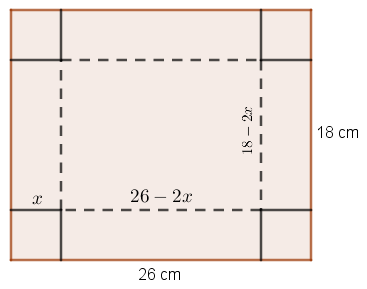
\includegraphics[width=2in]{TakeOutBox.png}

Find the volume of the box when $x = 2$.
\end{frame}

\begin{frame}[t]{Factoring Polynomials}
We just looked at expanding products of polynomials using multiplication.

When we factor, we are trying to write one a polynomial as the product of two or more polynomials.

Often, the terms in a polynomial will have a factor in common.

In this case, we can factor the polynomial by factoring out that common factor.
\end{frame}

\begin{frame}[t]{Factoring out Common Factors}
Factor each expression: \begin{enumerate}[(a)]
\item $5x^3 - 15x^2$
\item $-3 + 6x - 12x^3$
\item $(x+1)\fp{x^2} - (x+1)(2)$
\end{enumerate}
\end{frame}

\begin{frame}[t]{Factoring Special Forms}
Below are some common special polynomial forms. It is very important that you be comfortable factoring these going forward.

\pause

Difference of Squares: \\
$u^2 - v^2 = (u+v)(u-v)$

\pause

Perfect Square Trinomials: \\
$u^2 + 2uv + v^2 = (u + v)^2$ and $u^2 - 2uv + v^2 = (u - v)^2$

\pause

Sum and Difference of Two Cubes: \\
$u^3 + v^3 = (u+v)\fp{u^2 - uv + v^2}$ and $u^3 - v^3 = (u - v)\fp{u^2 + uv + v^2}$
\end{frame}

\begin{frame}[t]{Factoring Special Forms}
Factor $4x^2 - 81$.

\pause \vfill

Factor $a^2 + 16ab + 64b^2$.
\end{frame}

\begin{frame}[t]{Factoring Special Forms}
Factor $g^3 - 64$.

\pause \vfill

Factor $100 - 4y^2$.
\end{frame}

\begin{frame}[t]{Factoring by Grouping}
Sometimes, we can factor polynomials with more than three terms by grouping.

Example: Factor $x^3 + x^2 - 5x - 5$.

\pause \vfill

Example: Factor $x^3 - 3x^2 - 4x + 12$
\end{frame}

\begin{frame}[t]{Factoring Trinomials}
A trinomial has three terms, and we can often factor trinomials of the form $ax^2 + bx + c$.

I teach the ``ac" method of factoring, which involves factoring by grouping. \pause

In the ``ac" method of factoring, you complete the following steps: \begin{enumerate}[1)]
	\item<3-> Find a pair of numbers that multiplies to $a\times c$ and adds to $b$.
	\item<4-> Expand the polynomial using these two numbers.
	\item<5> Factor by grouping.
\end{enumerate}
\end{frame}

\begin{frame}[t]{Factoring Trinomials}
Factor $x^2 + 14x - 51$.

\vfill \pause

Factor $-6z^2 + 17z + 3$.
\end{frame}

\begin{frame}[t]{Next Steps}
\begin{itemize}
\item Complete Assignment \#1
\item Begin Module \#2
\begin{itemize}
\item Read Sections P.5 and P.6
\item Watch Video Lesson \#3
\end{itemize}
\end{itemize}
\end{frame}
\end{document}